\documentclass[11pt,a4paper]{article}
\usepackage[utf8]{inputenc}
\usepackage[vietnamese]{babel}
\usepackage{amsmath,amssymb}
\usepackage[version=4]{mhchem}
\usepackage{geometry}
\geometry{top=0.9cm,bottom=0.9cm,left=1.35cm,right=1.35cm,headheight=24pt,headsep=5pt,footskip=11pt}
\usepackage{graphicx}
\usepackage{xcolor}
\usepackage{tabularx}
\usepackage{array}
\usepackage{tikz}
\usepackage{multicol}
\usepackage{fancyhdr}
\usepackage{enumitem}

\definecolor{hfRed}{HTML}{D32F2F}
\definecolor{hfGreen}{HTML}{8BC390}
\definecolor{mainGreen}{HTML}{2E7D32}

\usepackage{ex_test}

\pagestyle{fancy}
\fancyhf{}
\renewcommand{\headrulewidth}{0.75pt}
\renewcommand{\headrule}{\hbox to\headwidth{\color{hfGreen}\leaders\hrule height \headrulewidth\hfill}}
\renewcommand{\footrulewidth}{0.75pt}
\renewcommand{\footrule}{\hbox to\headwidth{\color{hfGreen}\leaders\hrule height \footrulewidth\hfill}}

\fancyhead[L]{\small\itshape\color{hfRed}Tài liệu lưu hành nội bộ}
\fancyhead[R]{\small\color{hfRed}Thầy \textbf{TRẦN VĂN THẠNH} - 0777.470.803}

\fancyfoot[L]{\footnotesize\itshape\color{hfRed}CS1: 6/15 Nguyễn Hoàng, P. Kim Long, TP Huế \quad|\quad CS2: 24 Đặng Thái Thân, TP Huế}
\fancyfoot[R]{\small\textbf{\color{hfRed}Trang \thepage}}

\setlength{\parindent}{0pt}
\setlength{\parskip}{0.0pt}

\def\loigiai#1{}

\begin{document}
\Opensolutionfile{ans}[ans-de17-hs]

\noindent
\begin{minipage}[t]{0.48\textwidth}
	\textbf{SỞ GIÁO DỤC VÀ ĐÀO TẠO THỪA THIÊN HUẾ}\\
	\textbf{TRƯỜNG THPT HAI BÀ TRƯNG}\\
	\textbf{ĐỀ CHÍNH THỨC}\\
	\textit{(Đề thi có 04 trang)}
\end{minipage}\hfill
\begin{minipage}[t]{0.48\textwidth}
	\raggedleft
	\textbf{\color{mainGreen}ĐỀ KIỂM TRA ĐỊNH KỲ CHƯƠNG 6 (ĐẠI CƯƠNG KIM LOẠI)}\\
	\textbf{MÔN: HOÁ HỌC -- LỚP 12}\\
	\textit{Thời gian làm bài: 50 phút (không kể thời gian phát đề)}\\
	\textbf{Mã đề thi: 117}
\end{minipage}


\vspace{1pt}
\noindent\textit{Họ, tên thí sinh: \dots\dots\dots\dots\dots\dots\dots\dots\dots\dots\dots\dots\dots\dots\dots\dots\dots\dots\dots\dots\dots\dots Lớp: \dots\dots\dots\dots SBD: \dots\dots\dots\dots}\\
\noindent\textit{(Cho biết nguyên tử khối: H = 1; C = 12; N = 14; O = 16; Na = 23; Mg = 24; Al = 27; S = 32; Cl = 35,5; K = 39; Ca = 40; Fe = 56; Cu = 64; Zn = 65; Br = 80; Ag = 108; Ba = 137; Au = 197; Pb = 207; hằng số Faraday F = 96500 C/mol).}

\vspace{2pt}
\noindent
\textbf{PHẦN I (4,5 điểm -- 18 câu): Câu trắc nghiệm nhiều phương án lựa chọn.}\\
\textit{Thí sinh trả lời từ câu 1 đến câu 18. Mỗi câu hỏi thí sinh chỉ chọn một phương án.}

\setcounter{ex}{0}

\begin{ex}
Ở trạng thái cơ bản, cấu hình electron lớp ngoài cùng của nguyên tử Al ($Z = 13$) là
\choice
{$\ce{3s^1}$.}
{$\ce{3s^2}$.}
{$\ce{3s^2 3p^1}$.}
{$\ce{3p^1}$.}
\loigiai{}
\end{ex}

\begin{ex}
Ở trạng thái cơ bản, nguyên tử của nguyên tố nào sau đây có số electron lớp ngoài cùng ít nhất?
\choice
{C ($Z = 6$).}
{Li ($Z = 3$).}
{O ($Z = 8$).}
{F ($Z = 9$).}
\loigiai{}
\end{ex}

\begin{ex}
Ở trạng thái cơ bản, nguyên tử của nguyên tố nào sau đây có 3 electron ở lớp ngoài cùng?
\choice
{$_{11}\ce{Na}$.}
{$_{13}\ce{Al}$.}
{$_{20}\ce{Ca}$.}
{$_{26}\ce{Fe}$.}
\loigiai{}
\end{ex}

\begin{ex}
Thành phần nào sau đây \textbf{không} có trong mạng tinh thể kim loại?
\choice
{Ion kim loại.}
{Electron.}
{Nguyên tử kim loại.}
{Anion gốc acid.}
\loigiai{}
\end{ex}

\begin{ex}
Đốt một sợi dây kim loại X trong bình khí chlorine (\ce{Cl2}) thấy tạo ra khói màu nâu đỏ. X là kim loại nào sau đây?
\choice
{Mg.}
{Al.}
{Fe.}
{Cu.}
\loigiai{}
\end{ex}

\begin{ex}
Thuỷ ngân (Hg) là chất lỏng ở điều kiện thường, dễ bay hơi và hơi thuỷ ngân rất độc. Khi nhiệt kế thuỷ ngân bị vỡ, để tránh thuỷ ngân phân tán ra môi trường xung quanh, người ta gom thuỷ ngân lại rồi trộn với chất nào sau đây (ở dạng bột)?
\choice
{Carbon (C).}
{Magnesium (Mg).}
{Iron (Fe).}
{Sulfur (S).}
\loigiai{}
\end{ex}

\begin{ex}
Tính chất hoá học đặc trưng của kim loại là
\choice
{tính oxi hoá.}
{tính acid.}
{tính base.}
{tính khử.}
\loigiai{}
\end{ex}

\begin{ex}
Trong vỏ Trái Đất, kim loại nào sau đây có thể tồn tại ở dạng đơn chất?
\choice
{Na, Mg.}
{Al, Fe.}
{Cu, Zn.}
{Ag, Au.}
\loigiai{}
\end{ex}

\begin{ex}
Ion kim loại nào sau đây có nhiều nhất trong nước biển?
\choice
{\ce{Mg^2+}.}
{\ce{K+}.}
{\ce{Na+}.}
{\ce{Ca^2+}.}
\loigiai{}
\end{ex}

\begin{ex}
Hai nguyên tố kim loại phổ biến nhất trong vỏ Trái Đất là
\choice
{Mg, Ca.}
{Na, Ca.}
{Au, Ag.}
{Al, Fe.}
\loigiai{}
\end{ex}

\newpage

\begin{ex}
Nhôm (Al) là nguyên tố phổ biến thứ ba và là kim loại phổ biến nhất trong vỏ Trái Đất. Trong tự nhiên, quặng chính chứa nhôm là bauxite và quặng này là nguyên liệu chính để sản xuất nhôm trong công nghiệp. Thành phần chính của quặng bauxite là
\choice
{\ce{Na3AlF6}.}
{\ce{Al2O3.2H2O}.}
{\ce{KAl(SO4)2.12H2O}.}
{\ce{K2O.Al2O3.6SiO2}.}
\loigiai{}
\end{ex}

\begin{ex}
Hợp kim là vật liệu kim loại chứa một kim loại cơ bản với
\choice
{một số kim loại khác hoặc phi kim.}
{một số oxide của kim loại đó.}
{một số oxide kim loại khác hoặc phi kim.}
{một số phi kim và oxide của phi kim đó.}
\loigiai{}
\end{ex}

\begin{ex}
Phát biểu nào sau đây sai?
\choice
{Tính chất vật lí của hợp kim khác nhiều so với của đơn chất thành phần.}
{Tính chất hoá học của hợp kim tương tự tính chất của đơn chất thành phần.}
{Tính chất cơ học của hợp kim phụ thuộc vào thành phần đơn chất của hợp kim.}
{Tính chất cơ học của hợp kim không phụ thuộc vào hàm lượng các đơn chất.}
\loigiai{}
\end{ex}

\begin{ex}
Trường hợp nào sau đây đã sử dụng phương pháp điện hoá để chống ăn mòn kim loại?
\choice
{Mạ vàng lên quai đồng hồ.}
{Bôi dầu mỡ lên xích xe đạp.}
{Gắn tấm kẽm lên mặt ngoài vỏ tàu biển.}
{Sơn kín bề mặt khung cửa thép.}
\loigiai{}
\end{ex}

\begin{ex}
Trường hợp nào sau đây \textbf{không} xảy ra sự ăn mòn kim loại?
\choice
{Tàu đánh cá làm bằng thép bị hoen gỉ sau thời gian đi biển về.}
{Trống đồng bị chuyển màu xanh khi để lâu ngày trong không khí ẩm.}
{Vòng tay làm bằng bạc kim loại bị hoá đen khi sử dụng lâu ngày.}
{Nấu chảy vàng để đúc khuôn khi chế tác vàng trang sức.}
\loigiai{}
\end{ex}

\begin{ex}
Khi kim loại bị ăn mòn, luôn xảy ra quá trình nào sau đây?
\choice
{Oxi hoá kim loại thành ion kim loại.}
{Khử ion kim loại thành kim loại.}
{Khử oxygen trong không khí.}
{Khử kim loại thành ion kim loại.}
\loigiai{}
\end{ex}

\begin{ex}
Trường hợp nào sau đây kim loại bị phá huỷ chủ yếu do ăn mòn hoá học?
\choice
{Thiết bị làm bằng thép trong lò đốt lâu ngày bị phá huỷ.}
{Thép xây dựng bị gỉ khi để lâu ngày trong không khí ẩm.}
{Ống nước làm bằng gang bị gỉ khi chôn dưới đất lâu ngày.}
{Vỏ tàu biển làm bằng thép bị gỉ sau một thời gian sử dụng.}
\loigiai{}
\end{ex}

\begin{ex}
Trường hợp nào sau đây kim loại bị phá huỷ chủ yếu do ăn mòn điện hoá học?
\choice
{Thiết bị làm bằng sắt trong lò đốt lâu ngày bị phá huỷ.}
{Thước nhôm để trong không khí bị phủ bởi lớp \ce{Al2O3} ở bề mặt.}
{Cánh cửa làm bằng thép nhanh bị gỉ khi để ngoài trời mưa.}
{Đốt dây sắt trong bình khí chlorine.}
\loigiai{}
\end{ex}

\newpage

\noindent
\textbf{PHẦN II (4,0 điểm -- 4 câu): Câu trắc nghiệm đúng sai.}\\
\textit{Thí sinh trả lời từ câu 1 đến câu 4. Trong mỗi ý a), b), c), d) ở mỗi câu, thí sinh chọn đúng hoặc sai.}

\setcounter{ex}{0}

\begin{ex}
Tùy thuộc vào tính chất vật lí riêng của mỗi kim loại mà chúng được sử dụng vào những mục đích khác nhau. Mỗi phát biểu sau đây là đúng hay sai?
\choiceTF
{Kim loại chì (Pb) và cadmium (Cd) có nhiệt nóng chảy khá thấp nên được sử dụng làm dây chảy trong cầu chì.}
{Kim loại tungsten (W) có độ bền nhiệt và nhiệt độ nóng chảy rất cao nên được sử dụng làm dây tóc bóng đèn, thiết bị sưởi.}
{Do có tính dẻo và độ cứng phù hợp nên nhôm (Al) thường được gia công làm vật liệu như khung cửa, khung thiết bị.}
{Do kim loại magnesium (Mg) có khối lượng riêng là $1{,}735\text{ g/cm}^3$ nên được dùng để chế tạo các hợp kim nặng.}
\loigiai{}
\end{ex}

\begin{ex}
Đồng (Cu) là kim loại có tính khử yếu, không tan trong dung dịch \ce{H2SO4} loãng, nhưng tan được trong dung dịch \ce{H2SO4} đặc, nóng hoặc trong dung dịch \ce{H2SO4} loãng khi có mặt của \ce{O2} ngay ở nhiệt độ thường theo các phương trình hoá học sau:\\
(1) $\ce{Cu + 2H2SO4} \text{ (đặc, nóng)} \rightarrow \ce{CuSO4 + SO2 + 2H2O}$\\
(2) $\ce{2Cu + 2H2SO4} \text{ (loãng)} + \ce{O2} \rightarrow \ce{2CuSO4 + 2H2O}$\\
Mỗi phát biểu sau đây là đúng hay sai?
\choiceTF
{Trong hai phản ứng trên, \ce{H2SO4} đều đóng vai trò là chất oxi hoá.}
{Cùng một lượng \ce{CuSO4} tạo ra thì phản ứng (1) tiêu tốn \ce{H2SO4} nhiều hơn phản ứng (2).}
{Do có giá trị thế điện cực chuẩn dương nên Cu tác dụng được với dung dịch \ce{H2SO4} loãng ở (2).}
{Từ phản ứng (2) chứng tỏ $E^\circ_{\ce{Cu^2+/Cu}} < E^\circ_{\ce{O2, 4H+/2H2O}}$.}
\loigiai{}
\end{ex}

\begin{ex}
Cho các phát biểu sau về ứng dụng và tính chất của kim loại. Mỗi phát biểu sau đây là đúng hay sai?
\choiceTF
{Trong công nghiệp, nhôm được sản xuất bằng cách điện phân dung dịch \ce{AlCl3}.}
{Cho mẩu nhỏ Na vào dung dịch \ce{CuSO4}, thu được chất rắn là kim loại Cu.}
{Tái chế kim loại là giải pháp giúp con người sử dụng hiệu quả hơn nguồn tài nguyên.}
{Tất cả hợp kim của sắt đều dễ bị ăn mòn trong không khí ẩm.}
\loigiai{}
\end{ex}

\begin{ex}
Tiến hành thí nghiệm (như hình vẽ bên): Rót dung dịch \ce{NaCl} bão hoà vào cốc 1, cốc 2, cốc 3; cho dầu nhờn vào cốc 4. Cho vào cốc 1 và cốc 4 một đinh sắt sạch; cho vào cốc 2 đinh sắt sạch được quấn bởi dây kẽm; cho vào cốc 3 đinh sắt sạch được quấn bởi dây đồng. Để 4 cốc trong không khí khoảng 5 ngày.
\begin{center}
	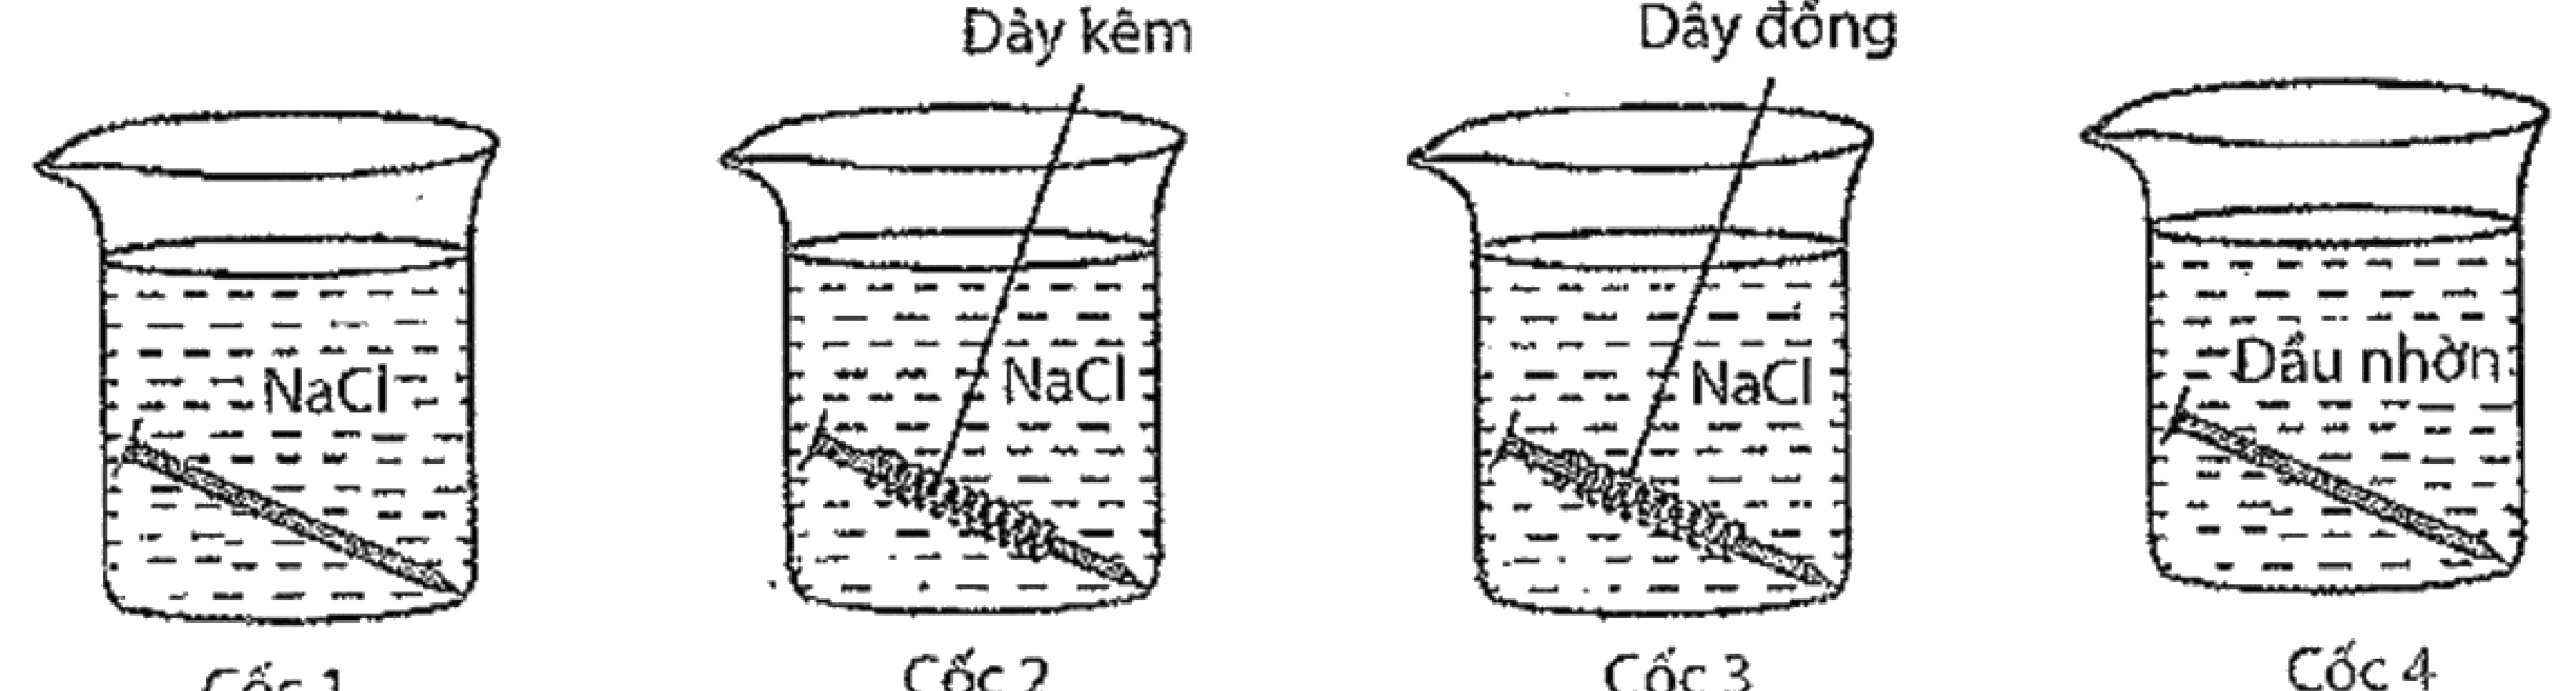
\includegraphics[width=0.68\textwidth]{images_crop_de17/p2_cau4_an_mon_sat.png}
\end{center}
Mỗi phát biểu sau đây là đúng hay sai?
\choiceTF
{Ở cốc 4, đinh sắt không bị gỉ (không bị ăn mòn).}
{Ở cốc 2, đinh sắt không bị gỉ, dây Zn bị ăn mòn và có khí thoát ra.}
{Ở cốc 3, đinh sắt bị gỉ nhiều nhất và dây đồng không bị ăn mòn.}
{Ở cốc 1, đinh sắt bị gỉ và dung dịch có màu vàng của \ce{FeCl2}.}
\loigiai{}
\end{ex}

\newpage

\noindent
\textbf{PHẦN III (1,5 điểm -- 6 câu): Câu trắc nghiệm yêu cầu trả lời ngắn.}\\
\textit{Thí sinh trả lời từ câu 1 đến câu 6.}

\setcounter{ex}{0}

\begin{ex}
Cho các nhận định sau:\\
(1) Các kim loại thuộc nhóm IA và IIA bao gồm các nguyên tố s.\\
(2) Nguyên tử của hầu hết các kim loại có từ 1 đến 3 electron ở lớp ngoài cùng.\\
(3) Nguyên tử kim loại dễ nhường electron hơn so với các nguyên tử phi kim.\\
(4) Trong mạng tinh thể kim loại, các electron chuyển động tự do theo nhiều hướng.\\
Có bao nhiêu nhận định là đúng?
\par\noindent\textit{Trả lời:} \dotfill
\loigiai{}
\end{ex}

\begin{ex}
Sắt (Fe) có số hiệu nguyên tử là 26. Trong vỏ Trái Đất, sắt là nguyên tố kim loại phổ biến thứ 2 (sau nhôm). Ứng dụng chủ yếu của sắt là để tạo ra các hợp kim thép dùng trong xây dựng và chế tạo. Cho các phát biểu sau:\\
(a) Ở trạng thái cơ bản, nguyên tử Fe có 6 electron ở lớp ngoài cùng.\\
(b) Hợp kim thép carbon khi để trong không khí ẩm sẽ bị ăn mòn điện hoá học.\\
(c) Trong vỏ Trái Đất, sắt tồn tại ở dạng hợp chất chủ yếu trong các quặng.\\
(d) Trong hợp chất, số oxi hoá của sắt chủ yếu là +2 và +3.\\
(e) Kim loại sắt (dư) tác dụng với chlorine tạo ra sản phẩm là \ce{FeCl2}.\\
Hãy cho biết có bao nhiêu phát biểu đúng trong các phát biểu trên.
\par\noindent\textit{Trả lời:} \dotfill
\loigiai{}
\end{ex}

\begin{ex}
Tiến hành các thí nghiệm:\\
(1) Đốt dây nhôm trong bình khí oxygen.\\
(2) Cho đinh thép sạch vào dung dịch \ce{H2SO4} loãng.\\
(3) Cho lá Al vào dung dịch \ce{CuSO4}.\\
(4) Nối dây nhôm với dây đồng rồi để trong không khí ẩm.\\
Liệt kê những thí nghiệm có xảy ra ăn mòn điện hoá học theo số thứ tự tăng dần (ví dụ: 1, 2, 3).
\par\noindent\textit{Trả lời:} \dotfill
\loigiai{}
\end{ex}

\begin{ex}
Để xảy ra ăn mòn điện hoá học thì cần đủ các yếu tố nào sau đây?\\
(1) Phải có hai điện cực khác chất nhau (hai kim loại khác nhau hoặc kim loại với phi kim).\\
(2) Hai điện cực phải tiếp xúc với nhau (trực tiếp hoặc gián tiếp qua dây dẫn).\\
(3) Hai điện cực phải được nối qua vôn kế hoặc ampe kế.\\
(4) Hai điện cực phải cùng tiếp xúc với một dung dịch chất điện li.\\
Liệt kê các yếu tố cần thiết theo số thứ tự tăng dần (ví dụ: 1, 2, 4).
\par\noindent\textit{Trả lời:} \dotfill
\loigiai{}
\end{ex}

\begin{ex}
Trong công nghiệp sản xuất gang ở nước ta hiện nay, muốn sản xuất ra 1 tấn gang cần phải sử dụng 1,7 đến 1,8 tấn quặng sắt, 0,6 đến 0,7 tấn đá vôi làm chất trợ dung, 0,6 đến 0,8 tấn than cốc. Giả thiết trong đá vôi \ce{CaCO3} chiếm 97\% khối lượng và 90\% than cốc chuyển hoá thành \ce{CO2}. Trong điều kiện sản xuất như trên, khi sản xuất được 1 tấn gang, nhà máy đã thải ra môi trường tối thiểu bao nhiêu $\text{m}^3$ khí \ce{CO2} ở điều kiện chuẩn? (Làm tròn kết quả đến hàng đơn vị).
\par\noindent\textit{Trả lời:} \dotfill
\loigiai{}
\end{ex}

\begin{ex}
Bằng phân tích quang phổ, người ta phát hiện trong “khí quyển” của sao Thuỷ có kim loại X. Biết X có cấu trúc mạng tinh thể lập phương tâm khối (độ đặc khít 68\%) và bán kính nguyên tử là $0{,}230\text{ nm}$. Khối lượng riêng của nguyên tố này là $0{,}862\text{ g/cm}^3$. (Biết Al = 27; K = 39; Zn = 65; Ba = 137). Xác định nguyên tử khối kim loại X.
\par\noindent\textit{Trả lời:} \dotfill
\loigiai{}
\end{ex}


\Closesolutionfile{ans}

\end{document}
